\documentclass{article}
\usepackage{amsmath}
\usepackage{amsfonts}
\usepackage{amssymb}
\usepackage{multicol}
\usepackage{graphicx}

\graphicspath{ {./images/} }

\setlength{\parindent}{0pt}

\begin{document}

\section{Antiderivatives}
An antiderivate $F(x)$ of $f(x)$ is defined by
\[F'(x) = f(x)\]
Notation for $F(x)$:
\[F(x) = \int f(x) \,dx\]
Some basic examples of antiderivatives:

\begin{multicols}{2}
    \begin{enumerate}
        \item $\int e^x \,dx = e^x+c$
        \item $\int 5x^2 \,dx = \frac{5}{3}x^3+c$
        \item $\int \sec^2(x) \,dx = \tan(x)+c$
    \end{enumerate}
\end{multicols}
List of antiderivates:
\begin{multicols}{2}
    \begin{enumerate}
        \item $\int x \,dx = \frac{x^{n+1}}{n+1} + c $
        \item $\int e^x \,dx = e^x +c$
        \item $\int \frac{1}{x} \,dx = \ln x+c$
        \item $\int n^x \,dx = \frac{n^x}{\ln n} +c$
        \item $\int \cos(x) \,dx = \sin(x) +c$
        \item $\int \sin(x) \,dx = -\cos(x) +c$
        \item $\int \sec^2(x) \,dx = \tan(x) +c$
        \item $\int \csc^2(x) \,dx = -\cot(x) +c$
        \item $\int \tan(x)\sec(x) \,dx = \sec(x) +c$
        \item $\int \cot(x)\csc(x) \,dx = -\csc(x) +c$
        \item $\int \frac{1}{\sqrt{1-x^2}} \,dx = \sin^{-1}(x) +c$
        \item $\int -\frac{1}{\sqrt{1-x^2}} \,dx = \cos^{-1}(x) +c$
        \item $\int \frac{1}{1+x^2} \,dx = \tan^{-1}(x) +c$
        \item $\int -\frac{1}{1+x^2} \,dx = \cot^{-1}(x) +c$
        \item $\int \frac{1}{x\sqrt{x^2-1}} \,dx = \sec^{-1}(x) +c$
        \item $\int -\frac{1}{x\sqrt{x^2-1}} \,dx = \csc^{-1}(x) +c$
    \end{enumerate}
\end{multicols}   

\section{Definite Integrals}
The definite integral of $f(x)$ from $a$ to $b$ is
\[\int_{a}^b f(x) \,dx = \sum_{k=1}^{n} f(c_{k})(x_k-x_{k-1})\]
where $\sum_{k=1}^{n} f(c_{k})(x_k-x_{k-1})$ is known as the \textbf{Riemann Sum}.

\subsection*{Area and Riemann Sum}
The Riemann Sum is an approximation of a region's area by adding up areas of multiple slices of the region.
\\\\
For example, given the graph of $y = 1-x^2$, we can imagine multiple rectangles of equal width and $n$ quantity as such:
\\
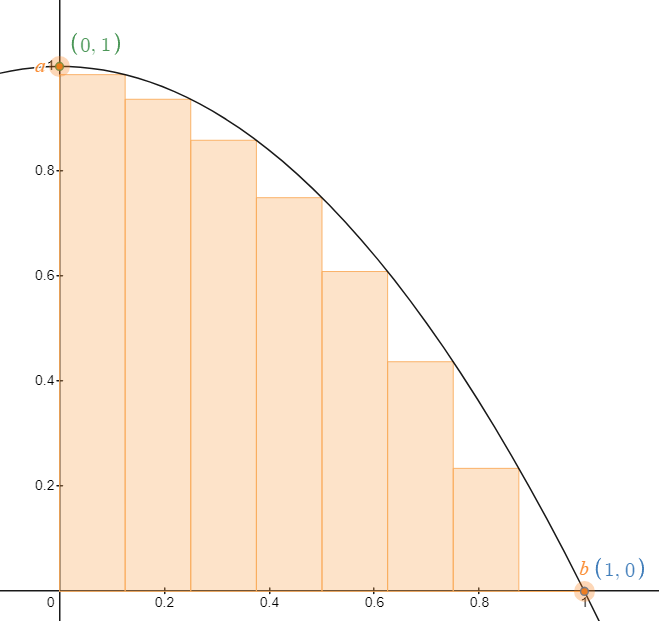
\includegraphics[width=7cm, height=5cm]{riemann2.PNG}
\\\\
Let the area of the rectangle be represented by
\[\Delta_k{A} = \text{area of the rectangle} = \text{length} \times \text{width} \]
Since the rectangles are of equal width, we can say that each rectangle has a width of
\[\Delta_k{x} = \frac{1}{n}\]
\\
We can then imagine each top-right corner of the rectangle to have the coordinates $(\frac{k}{n}, 1-(\frac{k}{n})^2)$ as shown:
\\
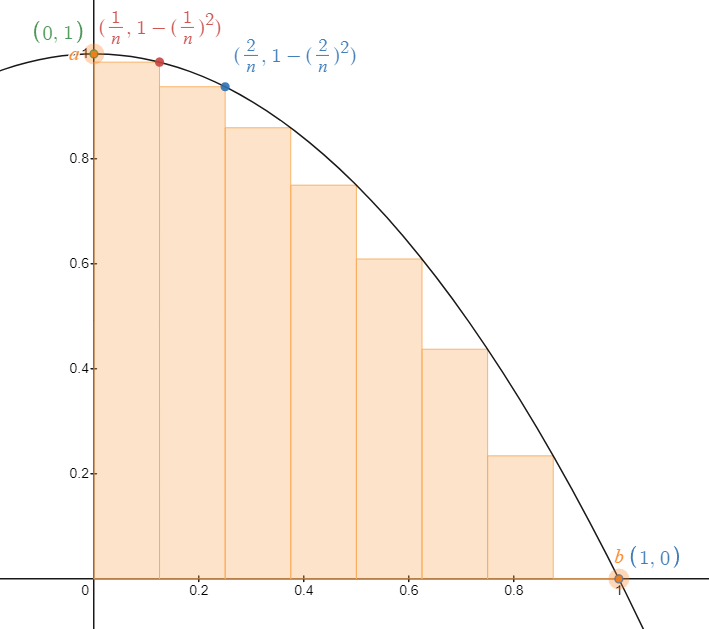
\includegraphics[width=7cm, height=5cm]{riemann1.PNG}
\\\\
Because of this, the area of each rectangle (for this specific graph) is:
\[\Delta_kA = 1-(\frac{k}{n})^2 \times \frac{1}{n}\]
\\
And the approximate area of all these rectangles is:
\[\Delta_{\text{Total}}A = \Delta_1A + \Delta_2A + \Delta_3A + ... + \Delta_nA\]
\\
This can be summarized as:
\[\sum_{k=1}^{n} \Delta_{k}A = \sum_{k=1}^{n} \, [1-(\frac{k}{n})^2](\frac{1}{n})\]
%\newpage
Since difference between approximate area and actual area gets smaller as more rectangles are added, we can find the actual area through:

\begin{align*}
    A &= \lim_{n \rightarrow \infty} \, \sum_{k=1}^{n} \, (1-\frac{k^2}{n^2})(\frac{1}{n}) \\
    &= \lim_{n \rightarrow \infty} \, (\frac{1}{n})( \sum_{k=1}^{n} \, 1 - \sum_{k=1}^{n} \, \frac{k^2}{n^2}) \\
    &= \lim_{n \rightarrow \infty} \, (\frac{1}{n})(n - \frac{1}{n^2} \sum_{k=1}^{n} \, k^2) && (\text{Since for the summation we only care about} \,k) \\
    &= \lim_{n \rightarrow \infty} \, (\frac{1}{n})(n - \frac{1}{n^2} (\frac{n(n+1)(2n+1)}{6})) && (\text{due to the sum of squares of natural numbers}) \\
    &= \lim_{n \rightarrow \infty} \, (\frac{1}{n})(n - \frac{n(n+1)(2n+1)}{6n}) \\
    &= \lim_{n \rightarrow \infty} \, 1 -\frac{(n+1)(2n+1)}{6n^2} \\
    &= \lim_{n \rightarrow \infty} \, 1 -\frac{2n^2+3n+1}{6n^2} \\
    &= \lim_{n \rightarrow \infty} \, 1 - \frac{2n^2}{6n^2} - \frac{3n}{6n^2} - \frac{1}{6n^2} \\
    &= 1 - \frac{1}{3} \\
    &= \frac{2}{3}
\end{align*}
\\
Note that using the power rule in integration yields the same result:
\[\int_{0}^{1} \, 1-x^2 \, dx = \left[x-\frac{x^2}{x}\right]_{0}^{1} = 1 - \frac{1}{3} = \frac{2}{3} \]

\subsection*{Properties of Definite Integrals}
\begin{flalign}
    \text{1.} \, &\int_{b}^{a}f(x)\,dx = \lim_{||\Delta||\rightarrow 0} \, \sum_{k=1}^{n} \, f(c_k)(x_k-x_k) && \\
    \text{2.} \, &\int_{b}^{a}f(x)\,dx = -\int_{a}^{b}f(x)\,dx && \\
    \text{3.} \, &\int_{a}^{a}f(x)\,dx = 0 && \\
    \text{4.} \, &\int_{a}^{b}f(x)\, dx = \int_{a}^{c}f(x)\, dx + \int_{c}^{b}f(x)\, dx \\\\
    \text{5.} \, &\text{Let } m \leq f(x) \leq M && \\
    &\forall x \text{ in } [a,b]\text{, then} && \\
    &m(b-a) \leq \int_{a}^{b}f(x)\, dx \leq M(b-a) && \\
    &m \leq \frac{1}{b-a} \int_{a}^{b}f(x)\, dx \leq M \hspace{20pt} (\text{average of } f \text{ over } [a,b]) && \\\\
    \text{6.} \, &\text{If } f(x) \leq g(x) \text{ on } [a,b] \text{, then} && \\
    & \int_{a}^{b}f(x)\, dx \leq \int_{a}^{b}g(x)\, dx && \\\\
    \text{7.} \, &\int_{a}^{b}f(x-k)\, dx = \int_{a+k}^{b+k}f(x)\, dx &&
\end{flalign}

\section{Fundamental Theorem of Calculus}

\section{Volume}
\subsection*{Method of Slices}
We can imagine an area element $A(x)$ or $A(y)$ that traverses through the solid vertically or horizontally. For example:
\\
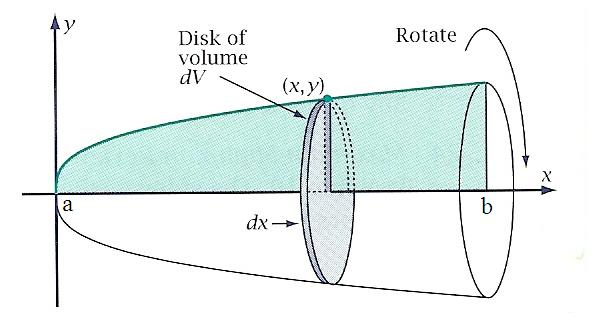
\includegraphics[scale=0.6]{volume1.jpeg}
\\
where volume is (with $A(x)$ being the area of the area element):
\[V = \int_{c}^{d} \, A(x) \, dx \]

\subsection*{Method of Disc/Washer}
\[V = \pi \int_{c}^{d} \, f(x)^2 \, dx \]

\subsection*{Method of Shells}

\end{document}

